% !TEX root = ../build-polygon/proof-recursion.tex



%%%%%%%%%%%%%%%%%%%%%%%%%%%%%%%%%%%%%%%%%%%%%%%%%%%%%%%%%%%%%%%%%%%%%%
\section{C12 PIL Description} \label{sec:c12}

Previously, we provided a brief overview of the high-level functioning of the \texttt{c12} arithmetization, highlighting its general properties and some insights of its PIL description. Now, our objective in this section is to provide a comprehensive and detailed explanation of the \texttt{c12} PIL arithmetization utilized during the generation and the constraining of the execution trace for the verification process of a FRI protocol.

\subsection{From \texttt{r1cs} to \plonk}

Recall that the verifier procedure verifying a generated STARK is written in \texttt{circom}. This procedure is responsible for constructing a set of \texttt{r1cs} (Rank-1 Constraint System) constraints.  Additionally, it is crucial to incorporate the utilization of custom gates that were specified earlier. Observe that custom gates are not directly checked in \texttt{circom} and the \texttt{.r1cs} file only contains computational information about its inputs and outputs. Consequently, the verification process for custom gates must be performed explicitly within the generated \texttt{pil} code that describes the verifier's verification procedure. The \texttt{pil} code will be responsible for incorporating the necessary validations for the custom gates, ensuring that they function as intended within the overall verification process. 

In contrast to \plonk constraints, it is not straightforward to translate \texttt{r1cs} constraints into a fixed column execution trace along with a set of \texttt{pil} constraints. Therefore, it becomes necessary to perform a conversion from \texttt{r1cs} constraints to \plonk ones in order to proceed. In what follows, we describe this conversion. 

Recall that a ($m$-dimensional) Rank-1 Constraint System (\texttt{r1cs}) over a set of signals $s_1, \dots, s_n$ is composed of three matrices $A = (a_{i, j}), B = (b_{i, j}),  C = (c_{i, j})$ each beloving to the matrix space $\mathrm{M}(m, n, \FF)$ where \FF represents the underlying field. We say that $s = (s_1, \dots, s_n)$ satisfy the constraints if and only if 
\[
As \circ Bs = Cs.
\]
where $\circ$ denotes the Hadamard product (or component-wise multiplication). More explicitly, $s_1, \dots, s_n$ satisfies the constraints if and only if
\begin{align*}
\left( a_{1, 1} s_1 + \dots + a_{1, n} s_n \right) &\cdot \left( b_{1, 1} s_1 + \dots + b_{1, n} s_n \right) = c_{1, 1} s_1 + \dots + c_{1, n} s_n \\
&\dots  \\
\left( a_{m, 1} s_1 + \dots + a_{m, n} s_n \right) &\cdot \left( b_{m, 1} s_1 + \dots + b_{m, n} s_n \right) = c_{m, 1} s_1 + \dots + c_{m, n} s_n \\
\end{align*}


Based on the previous explanation, it can be noted that the constraint $(1 + s_2) \cdot s_3 = s_4$ is not allowed in the R1CS formulation. In order to address the inclusion of constants in constraints, a designated signal $s_1$ is introduced to always maintain a value of $1$.

Notice that we can perceive \texttt{r1cs} constraints as gates with an unbounded fan-in (meaning they can have any number of input wires) and an unbounded fan-out (meaning they can have any number of output wires). This flexibility allows \texttt{r1cs} to accommodate a wide range of computations. On the other hand, \plonk gates operate with a fixed fan-in of $2$ (meaning that each gate has exactly two input wires) and fan-out of $1$ (meaning that each gate has exactly one output wire). A single \plonk gate with inputs signals $a, b$ and output signal $c$ is determined by $5$ selectors, namely $q_R, q_L, q_M, q_O$ and $q_C$ and we say that the tuple $(a, b, c)$ satisfies the gate equation if and only if
\[
a_R \cdot a + q_L \cdot b + q_M \cdot a \cdot b + q_O \cdot c + q_C = 0.
\]

The transformation process from a Rank-1 Constraint System to a set of \plonk constraints involves mapping each individual \texttt{r1cs} constraint to one or more \plonk constraints. To ensure a correct, optimized and comprehensive conversion, the reduction process can be divided into distinct cases, each addressing a specific scenario. Within each case, specific rules and mappings will be defined to convert the \texttt{r1cs} constraints into the appropriate \plonk constraints. These rules take into consideration the unique characteristics of each case, such as the types of variables involved, the operations performed, and the desired properties in the resulting \plonk constraints. The strategy for all of them consists on reducing sums adding constraints and variables. More specifically, consider the following linear combination $a_1 + a_2 s_2 + \dots + a_n s_n$, which has $n-1$ non-constant therms. We can reduce this linear combination to contain $n-2$ non-constant therms adding another artificial signal, say $v_1$, and the constraint $a_{n-1} s_{n-1} + a_n s_n = v_1$ (with the corresponding \plonk selectors $q_L = - a_{n-1}, q_R = - a_n, q_M = 0, q_O = 1$ and $q_C = 0$). Replacing this into the linear combination we get a new reduced linear combination $a_1 + a_2 s_2 + \dots + v_1$. We can perform the same strategy recursively to further reduce the linear combination to one having only two therms $a_1 + v_{T_a}$, where $T_a$ denotes the total number of newly added variables. Let us discuss the complete strategy for each of the cases:

\begin{itemize}


\item In constraints where $A = 0$ and/or $B = 0$, we get a linear constraint of the form
\[
c_{1} + c_{2} s_2 + \dots + c_{n} s_n = 0.
\]

The idea to optimally attack this case is to reduce apply the reduction strategy in order to reduce the number of additions to $4$ ($3$ non-constant factors and one reserved for the constant). More specifically, the reduced constraint will look like:
\[
c_1 + c_2 s_2 + c_3 s_3 + v_T = 0,
\]
where $T$ denotes the total amount of newly introduced signals. At this point we can directly convert the upper constraint into \plonk by setting $q_R = c_2, q_L = c_3, q_M = 0, q_O = 1$ and $q_C = c_1$. 

% Normalization is only in charge of deleting signals with constant equal to 0. 

\item In constraints with $a_i = 0$ except when $i = 1$ (corresponding exactly to the constant wire), we get a linear constraint of the form
\[
a_1 \cdot (b_{1} + b_{2} s_2 + \dots + b_{n} s_n) = c_{1} + c_{2} s_2 + \dots + c_{n} s_n.
\]

In this case,  In this case, the strategy is to multiply the constant $a_1$ with the linear combination and combine both sides of the equation:
\begin{align*}
&a_1 \cdot (b_{1} + b_{2} s_2 + \dots + b_{n} s_n) = c_{1} + c_{2} s_2 + \dots + c_{n} s_n \Longleftrightarrow \\
&a_1 b_1 + a_1 b_2 s_2 + \dots + a_1 b_n s_n  = c_{1} + c_{2} s_2 + \dots + c_{n} s_n \Longleftrightarrow \\
&a_1 b_1 + a_1 b_2 s_2 + \dots + a_1 b_n s_n - c_1 - c_2 s_2 - \dots - c_n s_n = 0
\end{align*}

Now, we proceed as before and we apply the reduction strategy in order to reduce the number of additions to $4$ ($3$ non-constant factors and one reserved for the constant). More specifically, the reduced constraint will look like:
\[
a_1 b_1 + a_1 b_2 s_2 + a_1 b_3 s_3 + a_1 v_T = 0,
\]
where $T$ denotes the total amount of newly introduced signals. At this point we can directly convert the upper constraint into \plonk by setting $q_R = a_1 \cdot b_2, q_L = a_1 \cdot b_3, q_M = 0, ¨q_O = a_1$ and $q_C = a_1 b_1$. 

\item In constraints with $b_i = 0$ except when $i = 1$ (corresponding exactly to the constant wire), we get a linear constraint of the form
\[
(a_{1} + a_{2} s_2 + \dots + a_{n} s_n) \cdot b_1 = c_{1} + c_{2} s_2 + \dots + c_{n} s_n.
\]

These constraints are handled symmetrically to the previous method described.

\item In this case fit all the other scenarios, so it deals with general constraints 
\[
(a_{1} + a_{2} s_2 + \dots + a_{n} s_n) \cdot (b_{1} + b_{2} s_2 + \dots + b_{n} s_n) = c_{1} + c_{2} s_2 + \dots + c_{n} s_n
\]
excluding the cases where each $a_i$ or $b_i$ is zero or where only $a_1$ (or $b_1$) differs from zero. In this case, the solution is to reduce each of the linear combinations to a single coefficient and a constant, say: 
\begin{align*}
&(a_1 + a \cdot v_{T_a}) \cdot (b_1 + b \cdot v_{T_b}) = c_1 + c \cdot v_{T_c} \Longleftrightarrow \\
&(a_1 + b_1 - c_1) + a_1 \cdot b  v_{T_b} + b_1 \cdot a \cdot v_{T_a} + a \cdot b \cdot v_{T_a} \cdot v_{T_b} - c \cdot v_{T_c} = 0
\end{align*}

We can directly convert the previous constraint to \plonk by setting $q_L = a \cdot b_1, q_R = a_1 \cdot b, q_M = a \cdot b, q_C = a_1 + b_1 - c_1$ and $q_O = -c$.  

\end{itemize}



\subsection{C12 Plonk Gates Verification}

Once the \texttt{r1cs} has been transformed into a set of \plonk constraints, we can proceed to generate an execution trace along with a corresponding \texttt{pil} file for its verification. To ensure optimal verification of the \POSEIDON custom gates, it is preferable to use an execution trace with a width of 12 columns. Consequently, the state update of a single round of a Poseidon hash can be verified by examining the transition between two rows, without requiring additional rows. 

However, when verifying regular \plonk gates in \texttt{pil} using 12 columns, we encounter a wastage of 7 constant columns. This wastage occurs because we only require 5 columns to accommodate the constants of the constraint. To address this issue, we can utilize 2 sets of constraints in each row, enabling the verification of 2 \plonk constraints within a single row. It's important to note that \plonk gates have a fan-in of 2 and a fan-out of 1. Consequently, by utilizing only 2 sets of signals per row, we end up wasting 6 witness columns. To address this issue, we can employ a technique that involves reusing constraints by utilizing the connection arguments available in \texttt{pil}. This approach allows us to optimize the allocation of witness columns and minimize wastage. 

The idea is simple. At a single row of our execution trace we will have two sets of \plonk constraints, namely $Q = \{ q_L, q_R, q_O, q_M, q_C \}$ and $Q' = \{ q_L', q_R', q_O', q_M', q_C' \}$. The initial six witness columns $(\acode[0], \dots, \acode[5])$ will correspond to $Q$, while the remaining six witness columns $(\acode[6], \dots, \acode[11])$ will relate to $Q'$. More specifically, the following constraints will be necessary to be fulfilled: 

\begin{align*}
&\acode[0] \cdot q_L + \acode[1] \cdot q_R + \acode[2] \cdot q_O + \acode[0] \cdot  \acode[1] \cdot q_M + q_C = 0 \\
&\acode[3] \cdot q_L + \acode[4] \cdot q_R + \acode[5] \cdot q_O + \acode[3] \cdot  \acode[4] \cdot q_M + q_C = 0 \\
&\acode[6] \cdot q_L' + \acode[7] \cdot q_R' + \acode[9] \cdot q_O' + \acode[6] \cdot  \acode[7] \cdot q_M' + q_C' = 0 \\
&\acode[9] \cdot q_L' + \acode[10] \cdot q_R' + \acode[11] \cdot q_O' + \acode[9] \cdot  \acode[10] \cdot q_M' + q_C' = 0
\end{align*}

In \texttt{pil} code, this is translated to:

\begin{pil}
pol a01 = a[0]*a[1];
pol g012 = C[3]*a01 + C[0]*a[0] + C[1]*a[1] + C[2]*a[2] + C[4];
g012*GATE = 0;

pol a34 = a[3]*a[4];
pol g345 = C[3]*a34 + C[0]*a[3] + C[1]*a[4] + C[2]*a[5] + C[4];
g345*GATE = 0;

pol a67 = a[6]*a[7];
pol g678 = C[9]*a67 + C[6]*a[6] + C[7]*a[7] + C[8]*a[8] + C[10];
g678*GATE = 0;

pol a910 = a[9]*a[10];
pol g91011 = C[9]*a910 + C[6]*a[9] + C[7]*a[10] + C[8]*a[11] + C[10];
g91011*GATE = 0;
\end{pil}

However, to ensure soundness and achieve the desired order of witness signals, we need to utilize connection arguments. These gates enable us to verify that the signals appearing in a specific \plonk constraint are accurate.

If we fail to assert this, the prover could incorrectly claim that:
\[
s_1 + s_2 = s_3 \quad \text{and} \quad s_4 - s_5 = s_6
\]
while the actual \plonk constraint is:
\[
s_4 + s_5 = s_6 \quad \text{and} \quad s_1 - s_2 = s_3
\]

Without ensuring the correct ordering of the witness signals, the prover could manipulate the equations and present an inaccurate representation of the \plonk constraint. By asserting the correct connection between the witness signals and the constraints, we prevent such incorrect claims and guarantee the accurate representation of the desired \plonk constraint. To establish this, we employ the following \texttt{pil} constraint:

\begin{pil}
{a[0], a[1], a[2], a[3], a[4], a[5], a[6], a[7], a[8], a[9], a[10], a[11]} connect
    {S[0], S[1], S[2], S[3], S[4], S[5], S[6], S[7], S[8], S[9], S[10], S[11]};
\end{pil}

where the $\texttt{S}$ polynomials keeps track of the exact permutation that corresponds to the position of the constraints we have deliberately placed along the execution trace.

\subsection{Poseidon Round Verification}

Whenever \POSEIDON is $1$, the PIL file will check that the vector 
\[
(\acode[0] \nextStep, \acode[1] \nextStep, \acode[2] \nextStep, \acode[3] \nextStep, \acode[4] \nextStep, \acode[5] \nextStep, \acode[6] \nextStep, \acode[7] \nextStep, \acode[8] \nextStep, \acode[9] \nextStep, \acode[10] \nextStep, \acode[11] \nextStep)
\]

is obtained applying the \texttt{POSEIDON} permutation to the vector
\[
(\acode[0], \acode[1], \acode[2], \acode[3], \acode[4], \acode[5], \acode[6], \acode[7], \acode[8], \acode[9], \acode[10], \acode[11]).
\]

Recall that the \texttt{POSEIDON} permutation has two modes: the partial permutation and the full one. The partial permutation is characterized by only-applying the S-Box layer to one element of the state (the first one, for example). However, a full round applies the S-Box to the whole set of $12$ elements which forms the state. Hence, we need a polynomial called \PARTIAL which will distinguish if the current round is a partial round or a full round. More concretely, \PARTIAL constant polynomial will be $1$ if and only if the current round is a partial round and $0$ otherwise. 

First of all, we will compute, if necessary, the $7$-th power of each element of the state in order to compute the S-Box layer. Moreover, we will add, at the beggining of the computation, the corresponding constant specified by the \texttt{Poseidon} permutation, which are stored in the polynomials \texttt{C[i]}. We will use the following code (written using \texttt{ejs}):

\begin{pil}
pol a<%- i %>_1 = a[<%- i %>] +  C[<%- i %>];
pol a<%- i %>_2 = a<%- i %>_1 * a<%- i %>_1;
pol a<%- i %>_4 = a<%- i %>_2 * a<%- i %>_2;
pol a<%- i %>_6 = a<%- i %>_4 * a<%- i %>_2;
pol a<%- i %>_7 = a<%- i %>_6 * a<%- i %>_1;
<%      if (i==0) { -%>
pol a<%- i %>_R = a<%- i %>_7;
<%      } else { -%>
pol a<%- i %>_R = PARTIAL * (a<%- i %>_1 - a<%- i %>_7) + a<%- i %>_7; 
<%      } -%>
<% } -%>
\end{pil}

We will carry $\texttt{ai\_R}$ to the next phase of the permutation to multiply it by the corresponding MDS matrix. Observe that we always exponentiate when $i=0$ (that is, the first element of the state). However, the other elements are only exponentiated if and only if \PARTIAL is $1$. The last part of the validation is trivial to validate:

\begin{pil}
POSEIDON12 * (a[0]'  - (25*a0_R + 15*a1_R + 41*a2_R + 16*a3_R +  2*a4_R + 28*a5_R + 13*a6_R + 13*a7_R + 39*a8_R + 18*a9_R + 34*a10_R + 20*a11_R)) = 0;
POSEIDON12 * (a[1]'  - (20*a0_R + 17*a1_R + 15*a2_R + 41*a3_R + 16*a4_R +  2*a5_R + 28*a6_R + 13*a7_R + 13*a8_R + 39*a9_R + 18*a10_R + 34*a11_R)) = 0;
POSEIDON12 * (a[2]'  - (34*a0_R + 20*a1_R + 17*a2_R + 15*a3_R + 41*a4_R + 16*a5_R +  2*a6_R + 28*a7_R + 13*a8_R + 13*a9_R + 39*a10_R + 18*a11_R)) = 0;
POSEIDON12 * (a[3]'  - (18*a0_R + 34*a1_R + 20*a2_R + 17*a3_R + 15*a4_R + 41*a5_R + 16*a6_R +  2*a7_R + 28*a8_R + 13*a9_R + 13*a10_R + 39*a11_R)) = 0;
POSEIDON12 * (a[4]'  - (39*a0_R + 18*a1_R + 34*a2_R + 20*a3_R + 17*a4_R + 15*a5_R + 41*a6_R + 16*a7_R +  2*a8_R + 28*a9_R + 13*a10_R + 13*a11_R)) = 0;
POSEIDON12 * (a[5]'  - (13*a0_R + 39*a1_R + 18*a2_R + 34*a3_R + 20*a4_R + 17*a5_R + 15*a6_R + 41*a7_R + 16*a8_R +  2*a9_R + 28*a10_R + 13*a11_R)) = 0;
POSEIDON12 * (a[6]'  - (13*a0_R + 13*a1_R + 39*a2_R + 18*a3_R + 34*a4_R + 20*a5_R + 17*a6_R + 15*a7_R + 41*a8_R + 16*a9_R +  2*a10_R + 28*a11_R)) = 0;
POSEIDON12 * (a[7]'  - (28*a0_R + 13*a1_R + 13*a2_R + 39*a3_R + 18*a4_R + 34*a5_R + 20*a6_R + 17*a7_R + 15*a8_R + 41*a9_R + 16*a10_R +  2*a11_R)) = 0;
POSEIDON12 * (a[8]'  - ( 2*a0_R + 28*a1_R + 13*a2_R + 13*a3_R + 39*a4_R + 18*a5_R + 34*a6_R + 20*a7_R + 17*a8_R + 15*a9_R + 41*a10_R + 16*a11_R)) = 0;
POSEIDON12 * (a[9]'  - (16*a0_R +  2*a1_R + 28*a2_R + 13*a3_R + 13*a4_R + 39*a5_R + 18*a6_R + 34*a7_R + 20*a8_R + 17*a9_R + 15*a10_R + 41*a11_R)) = 0;
POSEIDON12 * (a[10]' - (41*a0_R + 16*a1_R +  2*a2_R + 28*a3_R + 13*a4_R + 13*a5_R + 39*a6_R + 18*a7_R + 34*a8_R + 20*a9_R + 17*a10_R + 15*a11_R)) = 0;
POSEIDON12 * (a[11]' - (15*a0_R + 41*a1_R + 16*a2_R +  2*a3_R + 28*a4_R + 13*a5_R + 13*a6_R + 39*a7_R + 18*a8_R + 34*a9_R + 20*a10_R + 17*a11_R)) = 0;
\end{pil}

Numbers above are determined by the used MDS matrix of the permutation. More precisely, we are checking the matrix product shown below:
\setcounter{MaxMatrixCols}{20}
\[
\begin{pmatrix}
25 &15 &41 &16 &2 &28 &13 &13 &39 &18 &31 &20 \\
20 &17 &15 &41 &16 &2 &28 &13 &13 &39 &18 &34 \\
34 &20 &17 &15 &41 &16 &2 &28 &13 &13 &39 &18 \\
18 &34 &20 &17 &15 &41 &16 &2 &28 &13 &13 &39 \\
39 &18 &34 &20 &17 &15 &41 &16 &2 &28 &13 &13 \\
13 &39 &18 &34 &20 &17 &15 &41 &16 &2 &28 &13 \\
13 &13 &39 &18 &34 &20 &17 &15 &41 &16 &2 &28 \\
28 &13 &13 &39 &18 &34 &20 &17 &15 &41 &16 &2 \\
2  &28 &13 &13 &39 &18 &34 &20 &17 &15 &41 &16 \\
16 &2  &28 &13 &13 &39 &18 &34 &20 &17 &15 &41 \\
41 &16 &2  &28 &13 &13 &39 &18 &34 &20 &17 &15 \\
15 &41 &16 &2 &28 &13 &13 &39 &18 &34 &20 &17 
\end{pmatrix}
\cdot 
\begin{pmatrix}
\texttt{a0\_R} \\
\texttt{a1\_R} \\
\texttt{a2\_R} \\
\texttt{a3\_R} \\
\texttt{a4\_R} \\
\texttt{a5\_R} \\
\texttt{a6\_R} \\
\texttt{a7\_R} \\
\texttt{a8\_R} \\
\texttt{a9\_R} \\
\texttt{a10\_R} \\
\texttt{a11\_R}
\end{pmatrix}
= 
\begin{pmatrix}
\texttt{a[0]} \nextStep \\
\texttt{a[1]} \nextStep \\
\texttt{a[2]} \nextStep \\
\texttt{a[3]} \nextStep \\
\texttt{a[4]} \nextStep \\
\texttt{a[5]} \nextStep \\
\texttt{a[6]} \nextStep \\
\texttt{a[7]} \nextStep \\
\texttt{a[8]} \nextStep \\
\texttt{a[9]} \nextStep \\
\texttt{a[10]} \nextStep \\
\texttt{a[11} \nextStep
\end{pmatrix}
\]



\subsection{Extended Field Operations Verification} \label{sec:c12-cmuladd}

Whenever \CMULADD is $1$, the PIL file will check that the following elements of $\FF_{p^3}$
\begin{align*}
a &= \acode[0] + \acode[1] \cdot X + \acode[2] \cdot X^2 \\
b &= \acode[3] + \acode[4] \cdot X + \acode[5] \cdot X^2 \\
c &= \acode[6] + \acode[7] \cdot X + \acode[8] \cdot X^2 \\
\texttt{output} &= \acode[9] + \acode[10] \cdot X + \acode[11] \cdot X^2
\end{align*}
satisfy the relationship
\[
a \cdot b + c = \texttt{output}
\]
using the field operations inherited from 
\[
\FF_{p^3} \cong \FF_p[X]/(X^3 - X - 1).
\]

Given two elements $a_0 + a_1 X + a_2 X^2, b_0 + b_1 X + b_2 X^2 \in \FF_{p^3}$, we can express its product by computing the product of the polynomials, using Euclidean division and taking equivalence classes in $\FF_{p^3}$. It is not difficult to see, then, that we can express its product as
\begin{align*}
&(a_0 \cdot b_0 + a_1 \cdot b_2 + a_2 \cdot b_1) + \\
&(a_0 \cdot b_1 + a_1 \cdot b_0 + a_1 \cdot b_2 + a_2 \cdot b_1 + a_2 \cdot b_2) \cdot X + \\ 
&(a_0 \cdot b_2 + a_2 \cdot b_2 + a_2 \cdot b_0 + a_1 \cdot b_1) \cdot X^2
\end{align*}

Hence, the PIL code below states the correctness of the output elements $\acode[9], \acode[10], \acode[11]$ using polynomial relationships of degree less or equal than $2$ using the operation defined above:

\begin{pil}
pol cA = (a[0] + a[1]) * (b[0] + b[1]); 
pol cB = (a[0] + a[2]) * (b0 + b[2]);
pol cC = (a[1] + a[2]) * (b[1] + b[2]);
pol cD = a[0] * b[0];
pol cE = a[1] * b[1];
pol cF = a[2] * b[2];

CMULADD * (a[9] - (cC + cD - cE - cF) - c0) = 0;
CMULADD * (a[10] - (cA + cC - 2*cE - cD) - c1) = 0;
CMULADD * (a[11] - (cB - cD + cE) - c2) = 0;
\end{pil}

The previous piece of code works since:
\begin{align*}
&\texttt{cA} = (\texttt{a0} + \texttt{a1}) \cdot (\texttt{b0} + \texttt{b1}) = \texttt{a0} \cdot \texttt{b0} + \texttt{a0} \cdot \texttt{b1} + \texttt{a1} \cdot \texttt{b0} + \texttt{a1} \cdot \texttt{b1} \\
&\texttt{cB} = (\texttt{a0} + \texttt{a2}) \cdot (\texttt{b0} + \texttt{b2}) = \texttt{a0} \cdot \texttt{b0} + \texttt{a0} \cdot \texttt{b2} + \texttt{a2} \cdot \texttt{b0} + \texttt{a2} \cdot \texttt{b2} \\
&\texttt{cC} = (\texttt{a1} + \texttt{a2}) \cdot (\texttt{b1} + \texttt{b2}) = \texttt{a1} \cdot \texttt{b1} + \texttt{a1} \cdot \texttt{b2} + \texttt{a2} \cdot \texttt{b1} + \texttt{a2} \cdot \texttt{b2}
\end{align*}
Hence
\begin{align*}
&\acode[9] = \texttt{cC} + \texttt{cD} - \texttt{cE} - \texttt{cF} + \texttt{c0} = \texttt{a0} \cdot \texttt{b0} + \texttt{a1} \cdot \texttt{b2} + \texttt{a2} \cdot \texttt{b1} \\
&\acode[10] = \texttt{cA} + \texttt{cC} - 2 \texttt{cE} - \texttt{cD} + \texttt{c1} = \texttt{a0} \cdot \texttt{b1} + \texttt{a1} \cdot \texttt{b0} + \texttt{a1} \cdot \texttt{b2} + \texttt{a2} \cdot \texttt{b1} + \texttt{a2} \cdot \texttt{b2} \\
&\acode[11] = \texttt{cB} - \texttt{cD} + \texttt{cE} + \texttt{c2} = \texttt{a0} \cdot \texttt{b2} + \texttt{a2} \cdot \texttt{b2} + \texttt{a2} \cdot \texttt{b0} + \texttt{a1} \cdot \texttt{b1}
\end{align*}







\subsection{Fast Fourier Transform Verification}

Whenever \FFT is $1$, the PIL file will check the correct computation of a Fast Fourier Transform using the Coley-Tucker's butterfly method. Depending on the custom gate being validated, the input of the FFT can be $2$ elements or $4$ elements. Take into account that we apply the FFT to extended field elements, consisting on $3$ field elements. Depending on the number of input elements, the constants for the computation \CONST are adjusted in order to mimic the butterfly's formulas. Moreover, a parameter called \texttt{scale} is introduced in order to be able to perform inverse Fast Fourier Transforms. 

However, we should be able to perform much bigger FFTs, so the custom gate is programmed in order to optimize the computation using the necessary number of four-size FFT and, if necessary, complete them with the complementary number of two-sized FFT (observe that only $1$ of them may be necessary). Hence, we would also need a mechanism to chain them correspondingly following the butterfly diagram. 




\subsubsection{How to Chain FFTs}

First of all suppose that we want to perform the Fast Fourier Transform of $n$ elements in the base field $\FF_p$ where $n$ is a power of two having its exponent $\log_2(n)$ even. We are choosing a even exponent for the power of two since we will discuss first the case where no $2$-sized FFT are needed. The idea of the FFT is to reuse computations in order to reduce complexity. This can be seen easily using the butterfly diagram. Below, we will show the butterfly diagram for the case $n = 16$. We can reduce the total computation of the FFT for $16$ elements to a total amount of $8$ FFT of $4$ elements. However, chained FFT needs to be readapted and well-connected in order to express the correct computation. Observe that, before the first step, we should reverse the bits of the polynomial coefficients' indices in order to correctly order them all.


\begin{figure}[H]
\centering
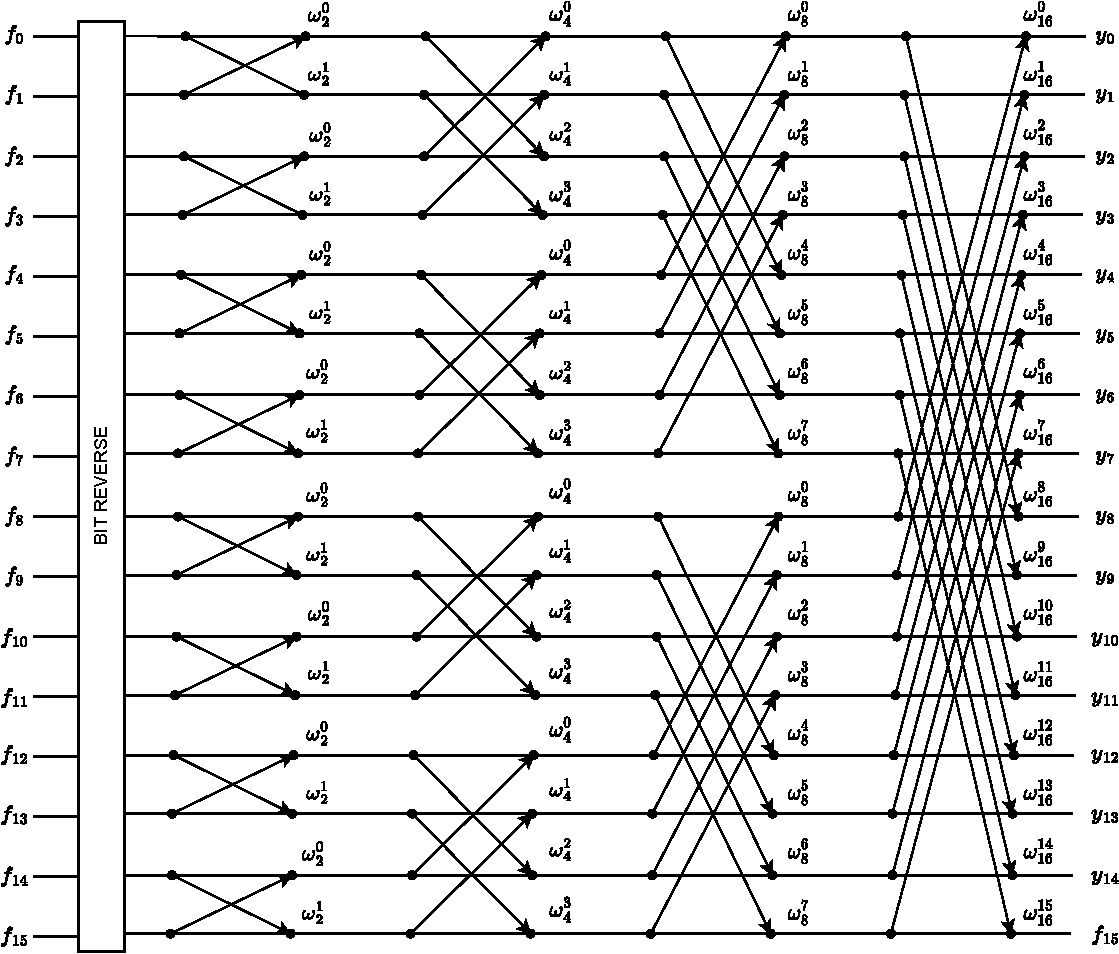
\includegraphics[width=0.77\textwidth]{\recursiondir/figures/16-elements-fft}
\caption{Butterfly diagram for 16 elements' Fast Fourier Transform.}
\label{fig:c12a-proof}
\end{figure}

Let us denote each of the $r + 1$ states of the $n$-sized Fast Fourier Transform as $(f_0^k, \dots, f_{n-1}^k)$, where $r = \log_2(n)$. The initial state $(f_0^0, \dots, f_{n-1}^0)$, representing the input, is labeled as step $0$, while the final state $(f_0^r, \dots, f_{n-1}^r)$, representing the output, is labeled as step $r$. Alternatively and aiming to clear pictures, we will also use $f_0, \dots, f_{n-1}$ for the input and $y_0, \dots, y_{n-1}$ for the output of the whole FFT. First of all, recall that, when fixing a certain step $k \in \{0, \dots, r - 1\}$, the next state $(f_0^{k+1} \dots, f_{n-1}^{k+1})$ of the butterfly structure can be directly computed from the previous one $(f_0^{k}, \dots, f_{n-1}^{k})$ as follows, for $j \in \{0, \dots, n/2 - 1\}$:
\begin{align*}
&f_j^{k+1} = f_j^k + f_{j + 2^k}^{k} \cdot \omega_{2^{k+1}}^j,                                           \\
&f_{j + 2^k}^{k+1} = f_j^k + f_{j + 2^k}^{k} \cdot \omega_{2^{k+1}}^{j + 2^k}
\end{align*}

being $\omega_{2^{k+1}} \in \FF_p^*$ a primitive $2^{k+1}$-root of unity. However, we can optimize the computation by exploiting the fact that:
\[
- \omega_{2^{k+1}}^j = \omega_{2^{k+1}}^{j + 2^k} \quad \text{ for } j \in \{0, \dots, 2^k - 1\}.
\]
By utilizing this property, we can avoid calculating half of the powers of $\omega_{2^{k+1}}$. Hence, we get the following optimized butterfly diagram:

\begin{figure}[H]
\centering
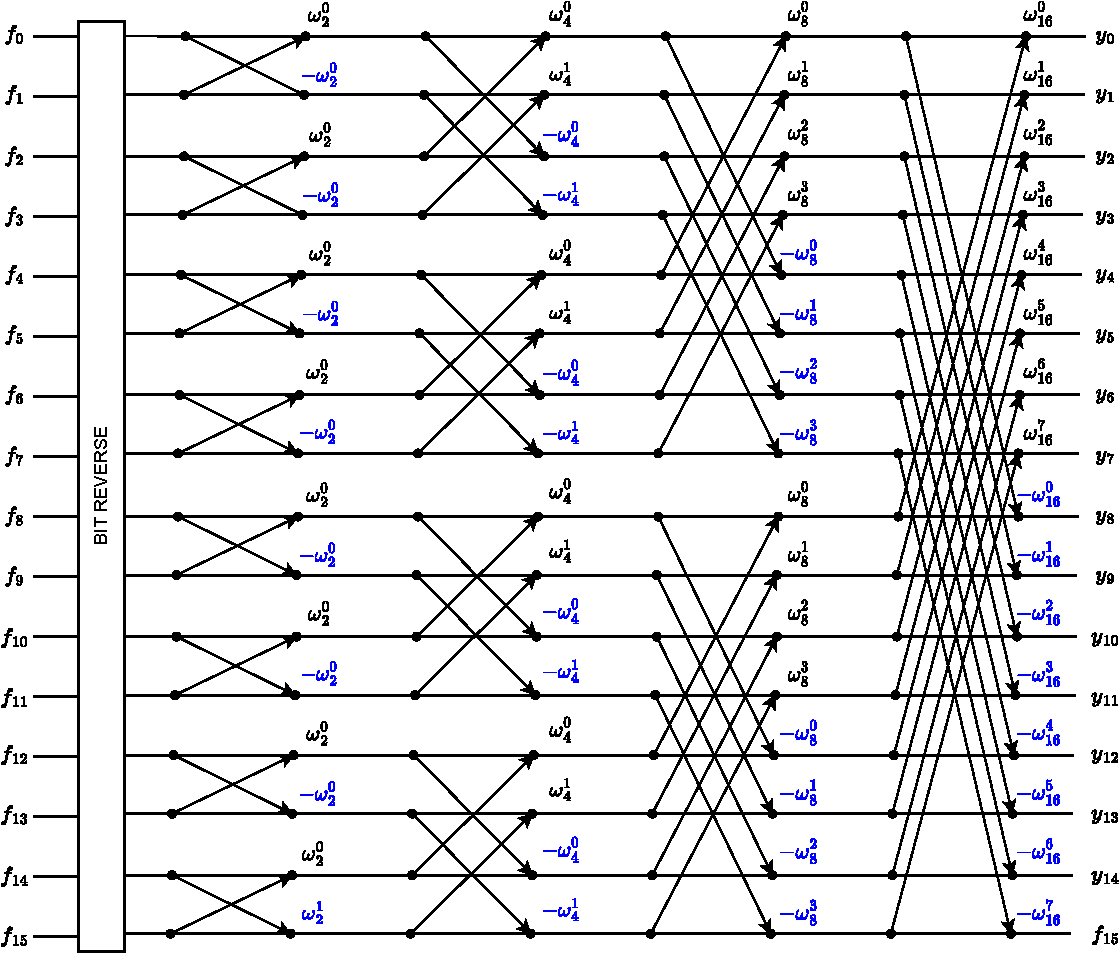
\includegraphics[width=0.77\textwidth]{\recursiondir/figures/optimized-16-elements-fft}
\caption{Optimized butterfly diagram for 16 elements' Fast Fourier Transform.}
\label{fig:c12a-proof}
\end{figure}

Hence, the previous formula for computing FFTs become the ones below, for each $j \in \{0, \dots, n/2 - 1\}$:
\begin{align*}
&f_j^{k+1} = f_j^k + f_{j + 2^k}^{k} \cdot \omega_{2^{k+1}}^j,                                           \\
&f_{j + 2^k}^{k+1} = f_j^k - f_{j + 2^k}^{k} \cdot \omega_{2^{k+1}}^j
\end{align*}

In the picture above it is important to observe some pattern. The components $y_0, y_4, y_8$ and $y_{12}$ of the output of the whole FFT of $16$ elements actually depend on the same intermediate $4$ coefficients $f_0^2, f_4^2, f_8^2, f_{12}^2$ appearing in the step $2$ of the FFT. In the picture below we show in red the wires that are connected to the components $y_0, y_4, y_8$ and $y_{12}$ and we can easily see that the previous statement is true. But this is not the only coincidence. 

\begin{figure}[H]
\centering
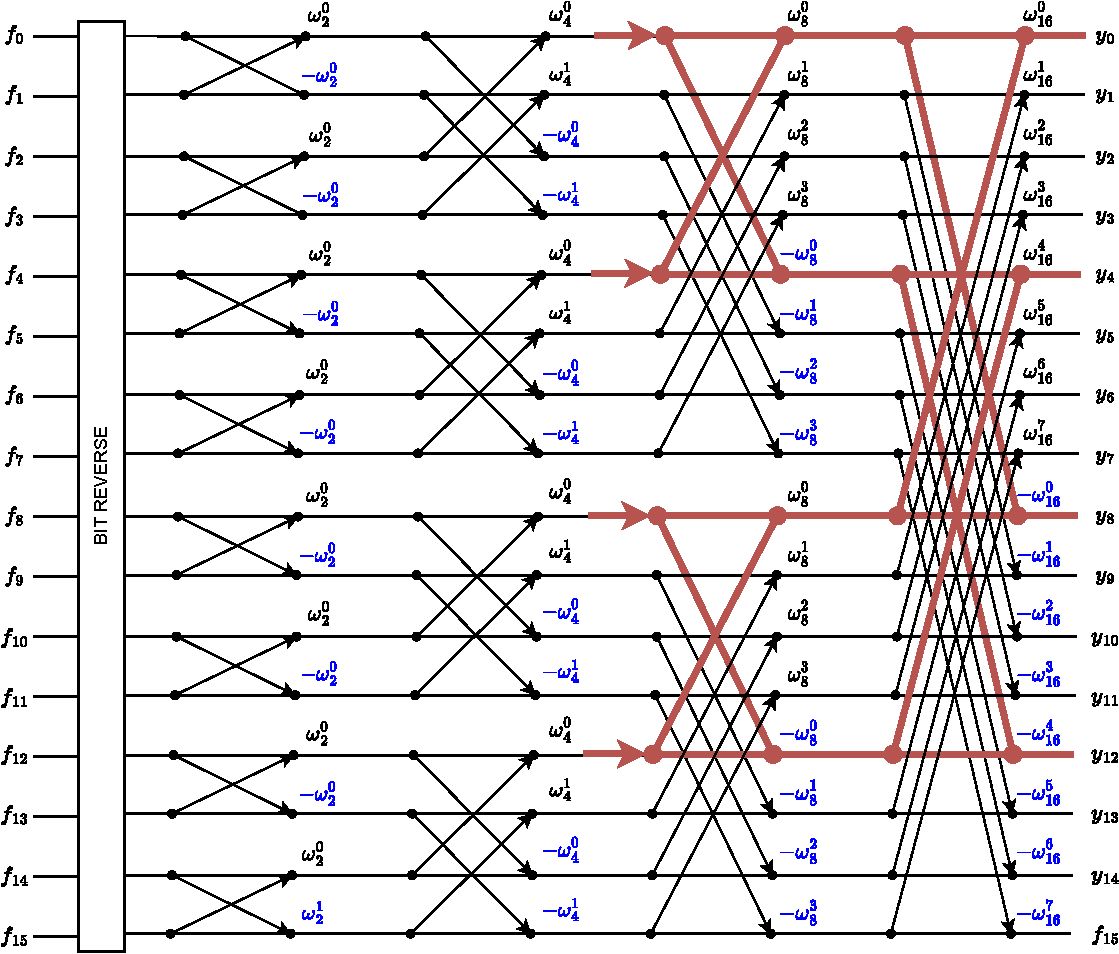
\includegraphics[width=0.77\textwidth]{\recursiondir/figures/16-elements-fft-connection}
\caption{Optimized butterfly diagram for 16 elements' Fast Fourier Transform.}
\label{fig:c12a-proof}
\end{figure}

Observe that, in fact, the subgraph formed by the red wires is actually another FFT of $4$ elements, with the output being $y_0, y_4, y_8$ and $y_{12}$. Therefore, $y_0, y_4, y_8$ and $y_{12}$ can be expressed as a linear combination of $f_0, f_4, f_8$ and $f_{12}$ having coefficients some convenient roots of unity. However, observe that, in this step, the used roots have to be modified accordingly. We depict the extracted subgraph in the figure below, in order to be able to see that in a clear way. 

\begin{figure}[H]
\centering
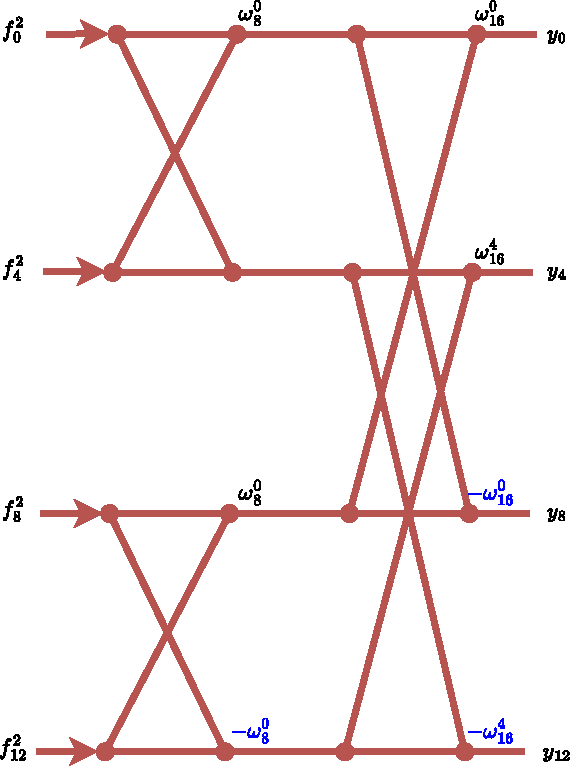
\includegraphics[width=0.5\textwidth]{\recursiondir/figures/fft-subgraph}
\caption{Subgraph representing a $4$-sized FFT chaining in the second step.}
\label{fig:c12a-proof}
\end{figure}

\newcommand{\bigslant}[2]{{\raisebox{.2em}{$#1$}\left/\raisebox{-.2em}{$#2$}\right.}}

In this case, the formulas to obtain $y_0, y_4, y_8$ and $y_{12}$ from $f_0^2, f_4^2, f_8^2$ and $f_{12}^2$ are the following:
\begin{align*}
y_0 &= f_0^3 + f_8^3 \cdot \omega_{16}^0  = (f_0^2 + f_4^2 \cdot \omega_{8}^0) + (f_8^2 + f_{12}^2 \cdot \omega_{8}^0) \cdot \omega_{16}^0          \\
    & = f_0^2 + f_4^2 \cdot \omega_8^0 + f_8^2 \cdot \omega_{16}^0 + f_{12}^2 \cdot \omega_8^0 \cdot \omega_{16}^0                                  \\
y_4 &= f_4^3 + f_{12}^3 \cdot \omega_{16}^4  = (f_0^2 - f_4^2 \cdot \omega_{8}^0) + (f_8^2 - f_{12}^2 \cdot \omega_{8}^0) \cdot \omega_{16}^4       \\
    & = f_0^2 - f_4^2 \cdot \omega_8^0 + f_8^2 \cdot \omega_{16}^4 - f_{12}^2 \cdot \omega_8^0 \cdot \omega_{16}^4                                  \\
y_8 &= f_0^3 - f_8^3 \cdot \omega_{16}^0  = (f_0^2 + f_4^2 \cdot \omega_{8}^0) - (f_8^2 + f_{12}^2 \cdot \omega_{8}^0) \cdot \omega_{16}^0          \\
    & = f_0^2 + f_4^2 \cdot \omega_8^0 - f_8^2 \cdot \omega_{16}^0 - f_{12}^2 \cdot \omega_8^0 \cdot \omega_{16}^0                                  \\
y_{12} &= f_4^3 - f_{12}^3 \cdot \omega_{16}^4  = (f_0^2 - f_4^2 \cdot \omega_{8}^0) - (f_8^2 - f_{12}^2 \cdot \omega_{8}^0) \cdot \omega_{16}^4    \\
    & = f_0^2 - f_4^2 \cdot \omega_8^0 - f_8^2 \cdot \omega_{16}^4 + f_{12}^2 \cdot \omega_8^0 \cdot \omega_{16}^4                                    
\end{align*}

To provide a more specific explaination, let's focus on determining the elements $f_j^k$ that belong to the same $4$-sized FFT at the step $k$, where $k$ is an even integer and $n$ is a power of $4$ (so that no $2$-sized FFT are needed at the end). Mathematically, we aim to compute a set of representatives for the classes of equivalence $\bigslant{\{f^k_j\}_{j=0}^{n-1}}{\thicksim^k}$, where $\thicksim^k$ denotes the equivalence relation $f_{j}^k \thicksim^k f_{j'}^k$ if they belong to the same $4$-sized FFT. Notice that if $f_j^{k+2}$ belongs to a equivalence class $f_j^k \in \bigslant{\{f^k_j\}_{j=0}^{n-1}}{\thicksim^k}$, where $j$ is the smallest index among all the elements in the class, then all the elements of its class can be expressed as:
\[
\left( f_{j}^{k}, f_{j + 2^{k} }^{k}, f_{j + 2 \cdot 2^{k}}^{k}, f_{j + 3 \cdot 2^{k}} ^{k} \right) 
\]


The equivalence relation in the set $\{f_0^k, \dots, f_{n-1}^k \}$ naturally induces an equivalence relation in the set of indices $\{0, \dots, n-1\}$. Therefore, we can interchangeably consider both perspectives. The first representative of each class is given by $f^k_{S_j^k}$, where $S_j^k$ is given by the sequence $\left( S_j^k \right)_j$ for $j \in \{0,\hdots,n/4-1\}$:
\begin{align*}
&S_j^k=S_{j-1}^k + 1                          &\text{if }S_{j-1}^k + 1 \not \equiv 0 \pmod{2^k} \\
&S_j^k=S_{j-1}^k + 3\cdot 2^k + 1           &\text{if }S_{j-1}^k + 1 \equiv 0 \pmod{2^k}
\end{align*}

Let us examine why the previous formula works more carefully. The following example provides a list of the corresponding indices for all the elements in each equivalence class, arranged in the natural order and computed by examining the butterfly diagram. This example considers the case of $n=64$ and $k=2$:

\begin{align*}
& (0,4,8,12), (1,5,9,13), (2,6,10,14), (3,7,1,15), \\
& (16, 20,21,28), (17,21,25,29), (18,22,26,30), (19,2,27,31), \\
& (32,36,40,44), (33,37,41,45), (34, 38, 42, 46), (35, 39, 43, 47), \\
& (48, 52, 56, 60), (49, 53, 57, 61), (50, 54, 58, 62), (51, 55, 59, 63)
\end{align*}
being each of the first representatives $S_j^k$ the following sequence of indexes
\[
0, 1, 2, 3, 16, 17, 18, 19, 32, 33, 34, 35, 48, 49, 50 \text{ and } 51.
\]


We notice that the sequence starts with $0, 1, 2, 3$, but there is an abrupt jump to $16$. Tis jump occurs because the index $4$ is already present in the class of $0$. Hence, we need to jump to the next free slot. We can compute this free slot from the last computed index, in this case $15$ (which is computed from $S_3^2$ as $S_3^2 + 3 \cdot 2^2$), and add one:
\[
S_4^2 = S_3^2 + 3 \cdot 2^2 + 1.
\]

To correctly determine all the values of $S_j^k$, it is essential to identify when these jumps occur. To do so, observe that we only need to check whether the consecutive index $S_{j-1}^k + 1$ is a multiple of $2^k$ or not. If $S_{j-1}^k + 1$ is a multiple, it indicates that $S_{j-1}^k + 1$ is already present in the computed classes.  In such cases, we need to compute the next index $S_j^k$ by adding $1$ to the last element of the current class, which is $S_{j-1}^k + 3 \cdot 2^k$. If not, we only need to add one to the current index, since the next one is not present yet. 


For instance, in the given example, we can see that $15$ satisfies the relation
\[
2^k = 2^2 = 4 \mid 4 = 3 + 1 = S_{3} + 1
\]
while
\begin{align*}
& 4 \nmid 1 = 0 + 1 = S_{0} + 1 \\
& 4 \nmid 2 = 1 + 1 = S_{1} + 1 \\
& 4 \nmid 3 = 2 + 1 = S_{2} + 1.
\end{align*}

Once we have defined the set of classes for each step $k$ of the FFT, we can compute the next state corresponding to step $k + 2$ by independently computing the $4$-sized FFT of each class. It's important to note that, since we are in the step $k$ of the $n$-sized FFT, we will need the values of $\omega_{2^k}$ and $\omega_{2^{k+1}}$. However, recall that we have the following fact:
\[
\omega_{2^{k+1}}^2 = \omega_{2^{k}}.
\]
For $k \in \{ 0, 2, \dots, \log_2(n) - 2 \}$, we can establish the following relationships:
\begin{align*}
& f_{S_j^k}^{k+2} = f_{S_j^k}^k + \omega_{2^{k+2}}^{\mathfrak{s}_j^k} \cdot f_{S_j^k + 2 \cdot 2^k}^k + \omega_{2^{k+2}}^{2{\mathfrak{s}_j^k}} \cdot f_{S_j^k + 2^k}^k + \omega_{2^{k+2}}^{3{\mathfrak{s}_j^k}} \cdot f_{S_j^k + 3 \cdot 2^k}^k \\
& f_{S_j^k + 2^{k}}^{k+2} = f_{S_j^k}^k + \omega_2 \cdot \omega_{2^{k+2}}^{\mathfrak{s}_j^k} \cdot f_{S_j^k + 2 \cdot 2^k}^k - \omega_{2^{k+2}}^{2{\mathfrak{s}_j^k}} \cdot f_{S_j^k + 2^k}^k  - \omega_2 \cdot \omega_{2^{k+2}}^{3{\mathfrak{s}_j^k}} \cdot f_{S_j^k + 3 \cdot 2^k}^k \\
& f_{S_j^k + 2 \cdot 2^{k}}^{k+2} = f_{S_j^k}^k - \omega_{2^{k+2}}^{\mathfrak{s}_j^k} \cdot f_{S_j^k + 2 \cdot 2^k}^k + \omega_{2^{k+2}}^{2{\mathfrak{s}_j^k}} \cdot f_{S_j^k + 2^k}^k - \omega_{2^{k+2}}^{3{\mathfrak{s}_j^k}} \cdot f_{S_j^k + 3 \cdot 2^k}^k \\
& f_{S_j^k + 3 \cdot 2^{k}}^{k+2} = f_{S_j^k}^k - \omega_2 \cdot \omega_{2^{k+2}}^{\mathfrak{s}_j^k} \cdot f_{S_j^k + 2 \cdot 2^k}^k - \omega_{2^{k+2}}^{2{\mathfrak{s}_j^k}} \cdot f_{S_j^k + 2^k}^k + \omega_2 \cdot \omega_{2^{k+2}}^{3{\mathfrak{s}_j^k}} \cdot f_{S_j^k + 3 \cdot 2^k}^k \\
\end{align*}
where 
\[
\mathfrak{s}_j^k = S_j^k \pmod{2^{k}}.
\]
The aforementioned equalities are derived from the fact that
\[
\omega^{j}_{2^{k+1}} \cdot \omega_2 = \omega^j_{2^{k+1}} \cdot \omega_{2^{k+1}}^{2k} =  \omega_{2^{k+1}}^{j + 2^k}
\]
which represents the two powers of $\omega_{2^{k+1}}$ associated with the same $4$-sized FFT class.

Now, let us move to the case where $n$ is an odd power of two (meaning that $\log_2(n)$ is odd). In the previous case, where $\log_2(n)$ is even, we only need to employ $4$-sized FFT chains. However, in this case, we must incorporate a final $2$-sized FFT step at the end of the whole process. At the last step, we will need to execute $n/2$ 2-sized FFTs, connecting $f_j^{r-1}$ and $f_{j+n/2}^{r-1}$ for $j \in \{ 0, \ldots, \frac{n}{2}-1 \}$. Thus, the formulas for the final step, applicable to $j \in \{ 0, \ldots, \frac{n}{2}-1 \}$, are as follows:
\begin{align*}
&f_j^{r} = f_j^{r-1} + f_{j+n/2}^{r-1} \cdot \omega_{n}^j \\
&f_{j+n/2}^{r} = f_{j+n/2}^{r-1} - f_{j}^{r-1} \cdot \omega_{n}^j
\end{align*}

Here, we have utilized the fact that $\omega_{n}^j = -\omega_{n}^{j+n/2}$.


\subsubsection{Fast Fourier Transform in Extension Fields}

In our case, it is important to emphasize that we are working with a cubic extension of the field $\mathbb{F}_p$. Therefore, in this section, we will explore the process of reducing the Fast Fourier Transform in an extension field to a number of FFTs equal to its degree, which is three in our case.


Supose that we want to compute the FFT of a polynomial with coeficients in a extension finite field $\FF_{p^r}$. Let $f(x)\in\FF_p$ be an irreducible polynomial with $\deg(f(x))=r$. We know that $\FF_{p^r}\cong \FF_{p}[x]/(f(x))$. Let $\{1,\hdots,\alpha^{r-1}\}$ be a $\FF_{p}$-basis, we can write any element $\beta\in\FF_{p^r}$ as $\beta=\sum_{i=1}^{r-1}a_i\cdot\alpha^{i}$.\\

Note that we can write any polynomial $p(x)\in\FF_{p^r}[x]$ as 
\[
p(x)=\sum_{j=1}^{n}\beta_jx^{j}=\sum_{j=1}^{n}\left(\sum_{i=1}^{r-1}a_j^i\alpha^{i}\right)x^{j}=\sum_{i=1}^{r-1}\alpha^i\left( \sum_{j=1}^{n}a_j^ix^n\right).
\]
Hence, in order to compute the FFT of $p(x)$, we only have to compute FFTs of the polynomials 
\[
p_i(x)=\sum_{j=1}^{n}a_j^ix^n
\] 
for $i\in\{1,\hdots,r-1\}$ (observe that $p_i(x)\in\FF_p[x]$).


\subsubsection{PIL Verification of the FFT}

Once we have described the chaining process for FFTs, let us describe how to verify its usage in PIL. We are given $12$ witness values, denoted as \acode{[0]}, \dots, \acode{[11]}. These values are used to form four extended field elements, namely $f_0, f_1, f_2, f_3 \in \FF_{p^3}$ constructed as follows:
\begin{align*}
&f_0 = \acode{[0]} + \acode{[1]} \cdot X + \acode{[2]} \cdot X^2 \\
&f_1 = \acode{[3]} + \acode{[4]} \cdot X + \acode{[5]} \cdot X^2 \\
&f_2 = \acode{[6]} + \acode{[7]} \cdot X + \acode{[8]} \cdot X^2 \\
&f_3 = \acode{[9]} + \acode{[10]} \cdot X + \acode{[11]} \cdot X^2
\end{align*}

Our goal is to verify whether the next row of witness values, denoted as $\acode[0] \nextStep, \dots, \acode[11] \nextStep$ mapped to the following extended field elements
\begin{align*}
&f_0 \nextStep = \acode[0] \nextStep + \acode[1] \nextStep \cdot X + \acode[2] \nextStep \cdot X^2 \\
&f_1 \nextStep = \acode[3] \nextStep + \acode[4] \nextStep \cdot X + \acode[5] \nextStep \cdot X^2 \\
&f_2 \nextStep = \acode[6] \nextStep + \acode[7] \nextStep \cdot X + \acode[8] \nextStep \cdot X^2 \\
&f_3 \nextStep = \acode[9] \nextStep + \acode[10] \nextStep \cdot X + \acode[11] \nextStep \cdot X^2
\end{align*}
satisfies the following relationship 
\[
(f_0 \nextStep, f_1 \nextStep, f_2 \nextStep, f_3 \nextStep) = \texttt{FFT4}(f_0 , f_1, f_2, f_3)
\]
where $\texttt{FFT4}(f_0, f_1, f_2, f_3)$ denotes the result of the $4$-sized Fast Fourier Transform of $f_0, f_1, f_2$ and $f_3$. Additionally, since we are chaining FFTs as explained earlier, we need to keep track of the current step of the $n$-sized FFT and its corresponding constants.

The polynomial constraints that need to be verified are of the following form:
\[
\FFT \cdot ( \acode[i] \nextStep - g_i) = 0
\]

Here, the selector $\FFT$ indicates that an FFT check is being performed, and $g_i$ represents a linear combination of the previous row of witness values, with coefficients determined by the current round. The coefficients correspond to the correct computation of the FFT.

To compute $g_i$, we set up constants denoted as $\texttt{C}[k]$ for different cases of FFT steps. Let's consider the cases where we perform a $4$-sized FFT and a $2$-sized FFT.

For a \textbf{$4$-sized FFT step}, the constants are:

\begin{align*}
& \texttt{C}[0] = 1 \\
& \texttt{C}[1] = \omega_{2^{k+2}}^{2{\mathfrak{s}_j^k}} \\
& \texttt{C}[2] = \omega_{2^{k+2}}^{{\mathfrak{s}_j^k}} \\
& \texttt{C}[3] = \omega_{2^{k+2}}^{3{\mathfrak{s}_j^k}} \\
& \texttt{C}[4]  = \omega_2 \cdot \omega_{2^{k+2}}^{{\mathfrak{s}_j^k}} \\
& \texttt{C}[5]  = \omega_2 \cdot \omega_{2^{k+2}}^{3{\mathfrak{s}_j^k}} \\
& \texttt{C}[6]  = 0 \\
& \texttt{C}[7]  = 0 \\
& \texttt{C}[8]  = 0 
\end{align*}

On the other hand, for a \textbf{$2$-sized FFT step} (that is, we are at the last step of a $n$-sized FFT with $n$ an odd power of two), we set up the constants as follows:

\begin{align*}
& \texttt{C}[0] = 0 \\
& \texttt{C}[1] = 0 \\
& \texttt{C}[2] = 0 \\
& \texttt{C}[3] = 0 \\
& \texttt{C}[4]  = 0 \\
& \texttt{C}[5]  = 0 \\
& \texttt{C}[6]  = 1\\
& \texttt{C}[7]  = \omega_{n}^j \\
& \texttt{C}[8]  = \omega_{n}^{j+1}
\end{align*}

To optimize the overall procedure, we employ a strategy that involves performing two consecutive $2$-sized FFTs at each step. This is achieved by utilizing two consecutive roots of unity within the constant values. This optimization approach proves to be optimal because the number of necessary $2$-sized FFTs doubles the amount of necessary $4$-sized FFTs, resulting in an efficient computation process.

Furthermore, we can introduce a scale factor of $1/n$ for each of the constants and change the corresponding root of unity to its inverse if we need to perform the inverse FFT. For a \textbf{$4$-sized FFT step}, the constants become:

\begin{align*}
& \texttt{C}[0] = 1/n \\
& \texttt{C}[1] = 1/n \cdot \omega_{2^{k+2}}^{-2{\mathfrak{s}_j^k}} \\
& \texttt{C}[2] = 1/n \cdot \omega_{2^{k+2}}^{-{\mathfrak{s}_j^k}} \\
& \texttt{C}[4]  = 1/n \cdot \omega_2 \cdot \omega_{2^{k+2}}^{-{\mathfrak{s}_j^k}} \\
& \texttt{C}[5]  = 1/n \cdot \omega_2 \cdot \omega_{2^{k+2}}^{-3{\mathfrak{s}_j^k}} \\
& \texttt{C}[6]  = 0 \\
& \texttt{C}[7]  = 0 \\
& \texttt{C}[8]  = 0 
\end{align*}

On the other hand, for a \textbf{$2$-sized FFT step}, we set up the constants as follows:

\begin{align*}
& \texttt{C}[0] = 0 \\
& \texttt{C}[1] = 0 \\
& \texttt{C}[2] = 0 \\
& \texttt{C}[3] = 0 \\
& \texttt{C}[4]  = 0 \\
& \texttt{C}[5]  = 0 \\
& \texttt{C}[6]  = 1/n \\
& \texttt{C}[7]  = 1/n \cdot \omega_{n}^{-j} \\
& \texttt{C}[8]  = 1/n \cdot \omega_{n}^{-j-1}
\end{align*}

Using these constants, we can compute the values of $g_i$ as follows:

\begin{pil}
pol g0  = C[0]*a[0] + C[1]*a[3] + C[2]*a[6] + C[3]*a[9]  + C[6]*a[0] + C[7]*a[3];
pol g3  = C[0]*a[0] - C[1]*a[3] + C[4]*a[6] - C[5]*a[9]  + C[6]*a[0] - C[7]*a[3];
pol g6  = C[0]*a[0] + C[1]*a[3] - C[2]*a[6] - C[3]*a[9]  + C[6]*a[6] + C[8]*a[9];
pol g9  = C[0]*a[0] - C[1]*a[3] - C[4]*a[6] + C[5]*a[9]  + C[6]*a[6] - C[8]*a[9];

pol g1  = C[0]*a[1] + C[1]*a[4] + C[2]*a[7] + C[3]*a[10] + C[6]*a[1] + C[7]*a[4];
pol g4  = C[0]*a[1] - C[1]*a[4] + C[4]*a[7] - C[5]*a[10] + C[6]*a[1] - C[7]*a[4];
pol g7  = C[0]*a[1] + C[1]*a[4] - C[2]*a[7] - C[3]*a[10] + C[6]*a[7] + C[8]*a[10];
pol g10 = C[0]*a[1] - C[1]*a[4] - C[4]*a[7] + C[5]*a[10] + C[6]*a[7] - C[8]*a[10];

pol g2  = C[0]*a[2] + C[1]*a[5] + C[2]*a[8] + C[3]*a[11] + C[6]*a[2] + C[7]*a[5];
pol g5  = C[0]*a[2] - C[1]*a[5] + C[4]*a[8] - C[5]*a[11] + C[6]*a[2] - C[7]*a[5];
pol g8  = C[0]*a[2] + C[1]*a[5] - C[2]*a[8] - C[3]*a[11] + C[6]*a[8] + C[8]*a[11];
pol g11 = C[0]*a[2] - C[1]*a[5] - C[4]*a[8] + C[5]*a[11] + C[6]*a[8] - C[8]*a[11];
\end{pil}

By checking these polynomial constraints, we can ensure the accuracy of the $n$-sized FFT computation for different scenarios, including both forward and inverse FFT, depending on the constants used. 

\subsection{Polynomial Evaluation Verification}

Whenever \EVPOL is $1$, the PIL file will check that the value 
\[
\acode[6] \nextStep + \acode[7] \nextStep \cdot X + \acode[8] \nextStep \cdot X^2 \in \FF_{p^3}
\]
is obtained by evaluating the polynomial
\[
p(Z) = \texttt{d0} \cdot Z^4 + \texttt{d1} \cdot Z^3 + \texttt{d2} \cdot Z^2 + \texttt{d3} \cdot Z + \texttt{d4}
\]
at a given point 
\[
z = \acode[3] \nextStep + \acode[4] \nextStep \cdot X + \acode[5] \nextStep \cdot X^2
\]
being \texttt{d0}, \texttt{d1}, \texttt{d2}, \texttt{d3} and \texttt{d4} $\in \FF_{p^3}$ defined as:
\begin{align*}
&\texttt{d0} = \acode[0] \nextStep + \acode[1] \nextStep \cdot X + \acode[2] \nextStep \cdot X^2 \\
&\texttt{d1} = \acode[9] + \acode[10] \cdot X + \acode[11] \cdot X^2 \\
&\texttt{d2} = \acode[6] + \acode[7] \cdot X + \acode[8] \cdot X^2   \\
&\texttt{d3} = \acode[3] + \acode[4] \cdot X + \acode[5] \cdot X^2   \\
&\texttt{d4} = \acode[0] + \acode[1] \cdot X + \acode[2] \cdot X^2
\end{align*}

This evaluation will be done using Horner's rule, so that $p(Z)$ will be rewritten as
\[
p(Z) = (((\texttt{d0} \cdot Z + \texttt{d1}) \cdot Z + \texttt{d2}) \cdot Z + \texttt{d3}) \cdot Z + \texttt{d4}.
\]
Also observe that all the operations performed at the evaluation are operations in $\FF_{p^3}$, so we will perform the operations in PIL using the following \texttt{CMulAdd} function, written in \texttt{ejs}. Observe that the logic is exactly the same than the one presented in Section \ref{sec:c12-cmuladd}.

Note that the order selected to input the parameters of the \EVPOL gate is totally arbitrary and we should only have to take care that is \textbf{completely} aligned with the Circom's custom gate. Moreover, observe that, since there are more than $12$ parameters, they all not fit in a row of the execution trace, forcing us to use $2$ of them to include them. This is not even a problem since the validation only occupies $3$ columns. 

\begin{js}
<% function CMulAdd(s, a0, a1, a2, b0, b1, b2, c0, c1, c2) {
    const code = [];
    code.push(`pol A${s} = (${a0} + ${a1})  * (${b0} + ${b1});`);
    code.push(`pol B${s} = (${a0} + ${a2})  * (${b0} + ${b2});`);
    code.push(`pol C${s} = (${a1} + ${a2})  * (${b1} + ${b2});`);
    code.push(`pol D${s} = ${a0} * ${b0};`);
    code.push(`pol E${s} = ${a1} * ${b1};`);
    code.push(`pol F${s} = ${a2} * ${b2};`);
    code.push(`pol acc${s}_0 = C${s}+ D${s} - E${s} - F${s} + ${c0};`);
    code.push(`pol acc${s}_1 = A${s}+ C${s}- 2*E${s} - D${s} + ${c1};`);
    code.push(`pol acc${s}_2 = B${s}- D${s} + E${s} + ${c2};`);
    code.push(`\n`);
    return code.join("\n");
} -%>
\end{js}

Now, we can compute $p(z) \in \FF_{p^3}$ using the previous function, accumulating the results by using the Horner's rule:

\begin{js}
// acc = d0 * x + d1 
<%- CMulAdd(
        "1", 
        "a[0]'", 
        "a[1]'", 
        "a[2]'", 
        "a[3]'", 
        "a[4]'", 
        "a[5]'", 
        "a[9]", 
        "a[10]", 
        "a[11]"
    ) 
-%>
\end{js}

\begin{js}
// acc2 = acc * x + d2 
<%- CMulAdd(
        "2",
        "acc1_0", 
        "acc1_1", 
        "acc1_2", 
        "a[3]'", 
        "a[4]'", 
        "a[5]'", 
        "a[6]'", 
        "a[7]", 
        "a[8]"
    ) 
-%>
\end{js}

\begin{js}
// acc3 = acc2 * x + d3 
<%- CMulAdd(
        "3", 
        "acc2_0", 
        "acc2_1", 
        "acc2_2", 
        "a[3]'", 
        "a[4]'", 
        "a[5]'", 
        "a[3]", 
        "a[4]", 
        "a[5]"
    ) 
-%>
\end{js}

\begin{js}
// acc4 = acc3 * x + d4 
<%- CMulAdd(
        "4", 
        "acc3_0", 
        "acc3_1", 
        "acc3_2", 
        "a[3]'", 
        "a[4]'", 
        "a[5]'", 
        "a[0]", 
        "a[1]", 
        "a[2]"
    ) 
-%>
\end{js}

Now, the only what remains is to check that the last values obtained $\texttt{acc3\_0}, \texttt{acc3\_1}, \texttt{acc3\_2}$ are equal to the supposed committed evaluation of $p$ at $z$, $\acode[6] \nextStep, \acode[7] \nextStep$ and $\acode[8] \nextStep$ respectively:

\begin{pil}
EVPOL4 * (a[6]' - acc4_0) = 0;
EVPOL4 * (a[7]' - acc4_1) = 0;
EVPOL4 * (a[8]' - acc4_2) = 0;
\end{pil}